\subsection{Global K-Means}
We have tested on each dataset 171 different configurations of the Global K-Means algorithm, by using the 3 different distance metrics with 19 different values of the k (from 2 to 20), and 3 different values for the number of buckets (2k, 3k and 4k). This time, we have only run the Global K-Means once for each of these configurations, since it is a deterministic algorithm that would return the same results every time. From the evaluation metrics extracted for each of these runs, we study the effect of each of the 3 hyperparameters and study the best performing runs according to each of the metrics.

\subsubsection{Hyperparameter Study}
As in the previous section, we start by observing some preliminary patterns about the effect of each hyperparameter on the clustering performance.

In Figure \ref{fig:globalkmeans:violin} we summarize the observed trends in each of the datasets (columns) for each of the hyperparameters (rows) with different metrics. It is not surprising to see that the patterns regarding the K-Means hyperparameters (k and distance metric) mostly repeat for the Global K-Means, since Global K-Means is mearly a modification of the same idea as the standard K-Means.

\begin{itemize}
    \item In the first row of plots, we observe that Hepatitis again favors low values of k; Mushroom does not achieve very conclusive results, but definitely gets consistently worse with higher values of k; and Pen-based benefits from intermediate values, getting more inconsistent for the highest ones.
    \item In the middle row, it is evident that the Clark distance performs significantly better on the Hepatitis dataset and significantly worse on the other 2 datasets, which are similar conclusions as we had reached before.
    \item In the last row, we observe that the clustering performance generally does not seem to be significantly altered by the different values of the number of buckets that we use to initilize the candidate points of the algorithm.
\end{itemize}


\begin{figure}[h]
    \centering
    \begin{tabular}{ccc}
        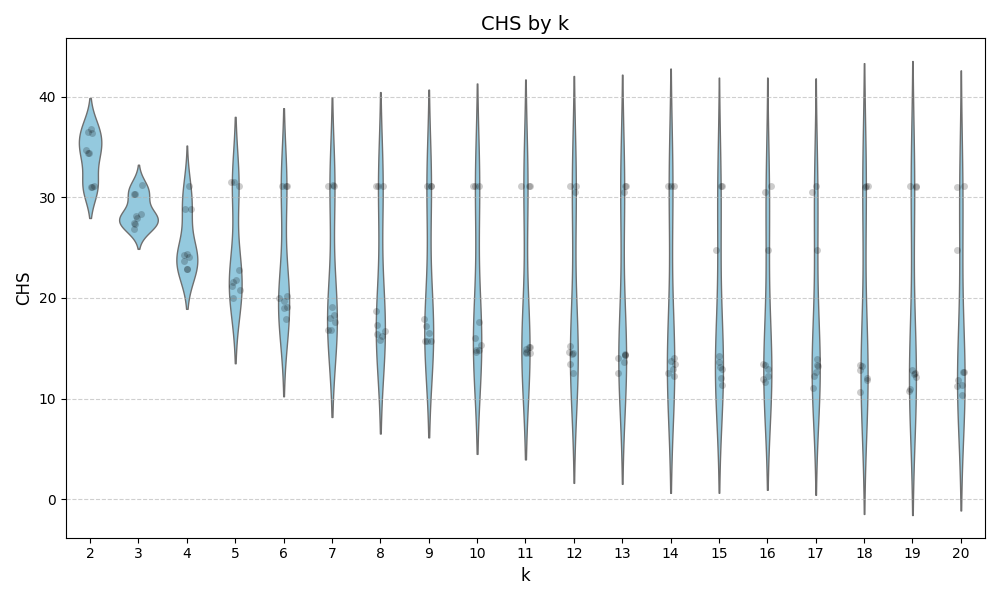
\includegraphics[width=0.3\textwidth]{figures/GlobalKMeans/hepatitis_violin_k_vs_CHS.png} & 
        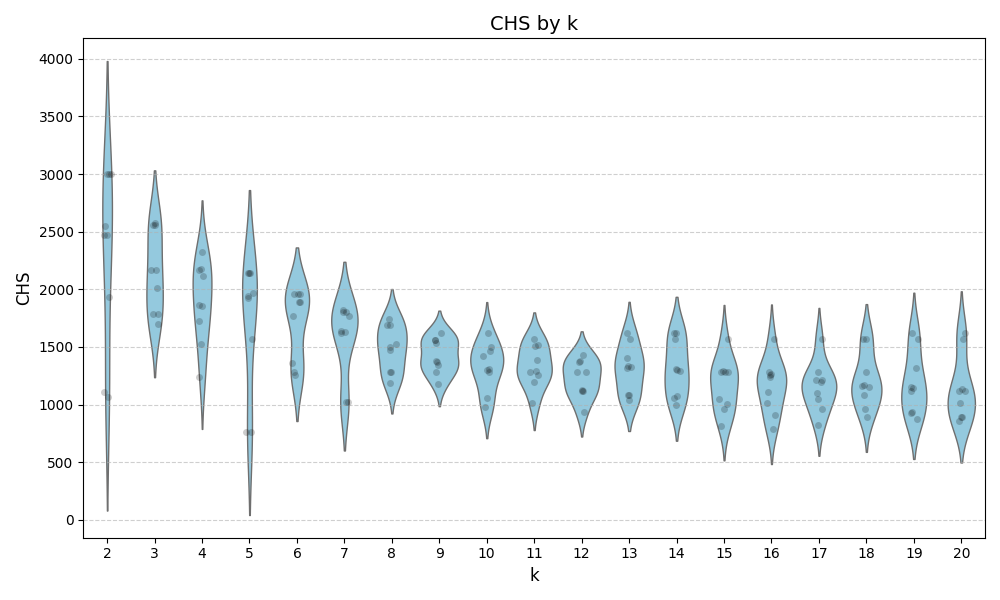
\includegraphics[width=0.3\textwidth]{figures/GlobalKMeans/mushroom_violin_k_vs_CHS.png} & 
        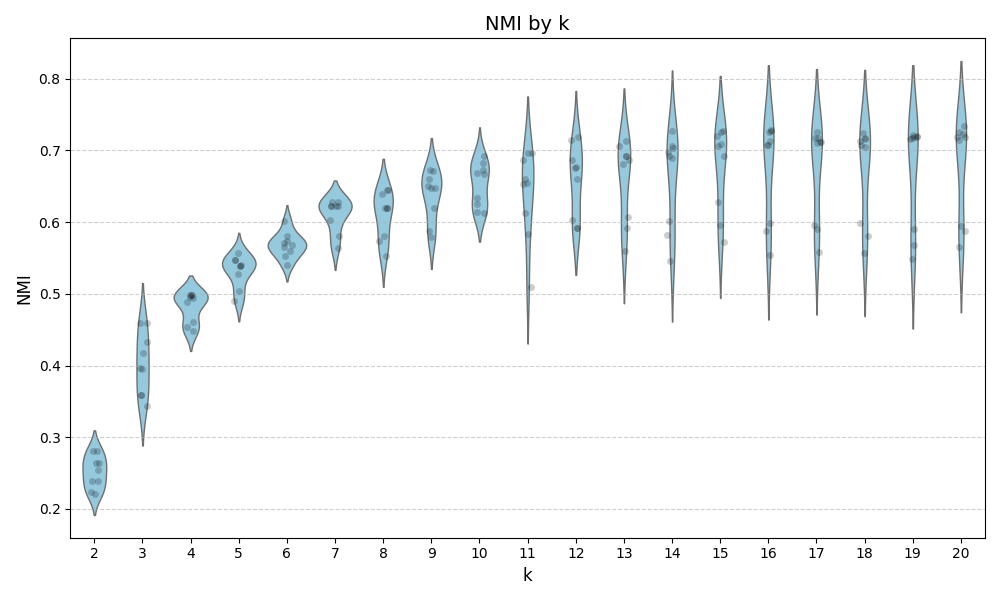
\includegraphics[width=0.3\textwidth]{figures/GlobalKMeans/penbased_violin_k_vs_NMI.png} \\
        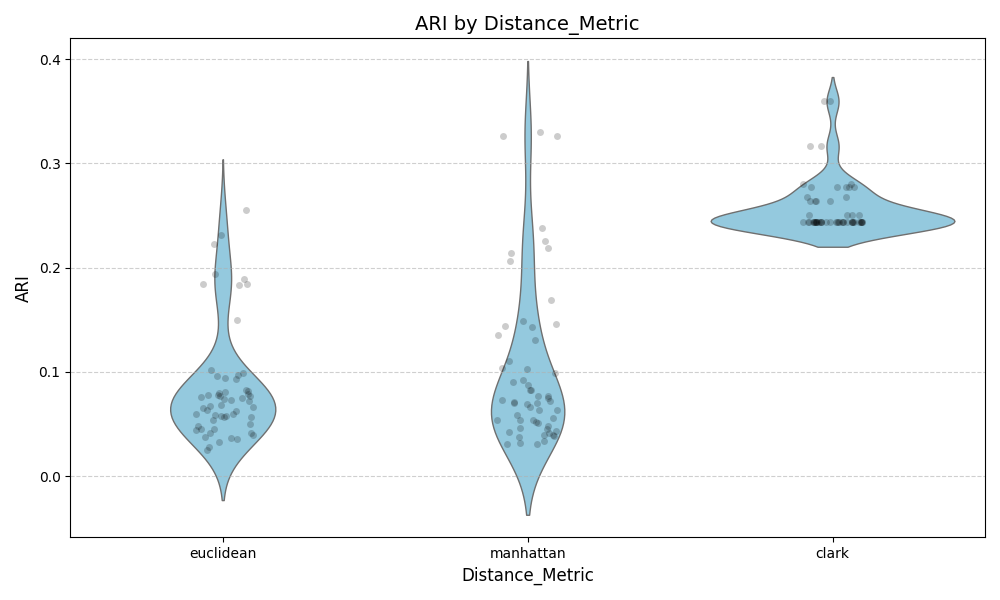
\includegraphics[width=0.3\textwidth]{figures/GlobalKMeans/hepatitis_violin_Distance_Metric_vs_ARI.png} & 
        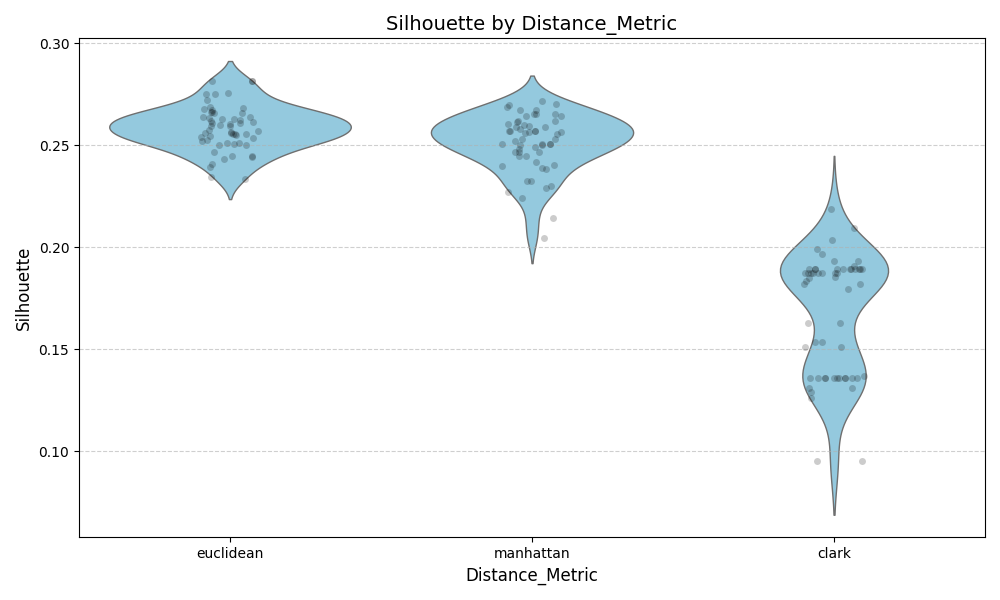
\includegraphics[width=0.3\textwidth]{figures/GlobalKMeans/mushroom_violin_Distance_Metric_vs_Silhouette.png} & 
        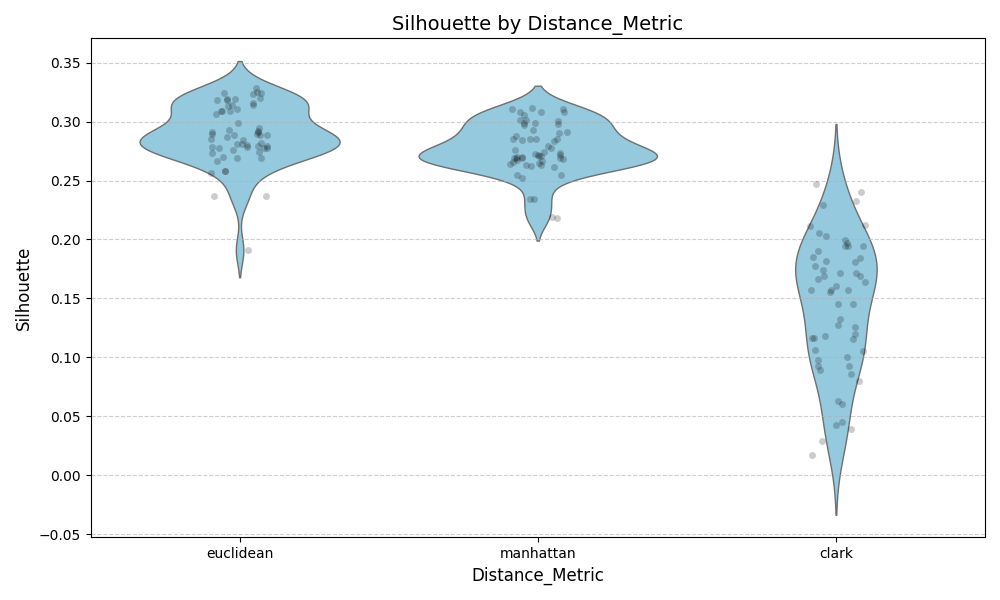
\includegraphics[width=0.3\textwidth]{figures/GlobalKMeans/penbased_violin_Distance_Metric_vs_Silhouette.png} \\
        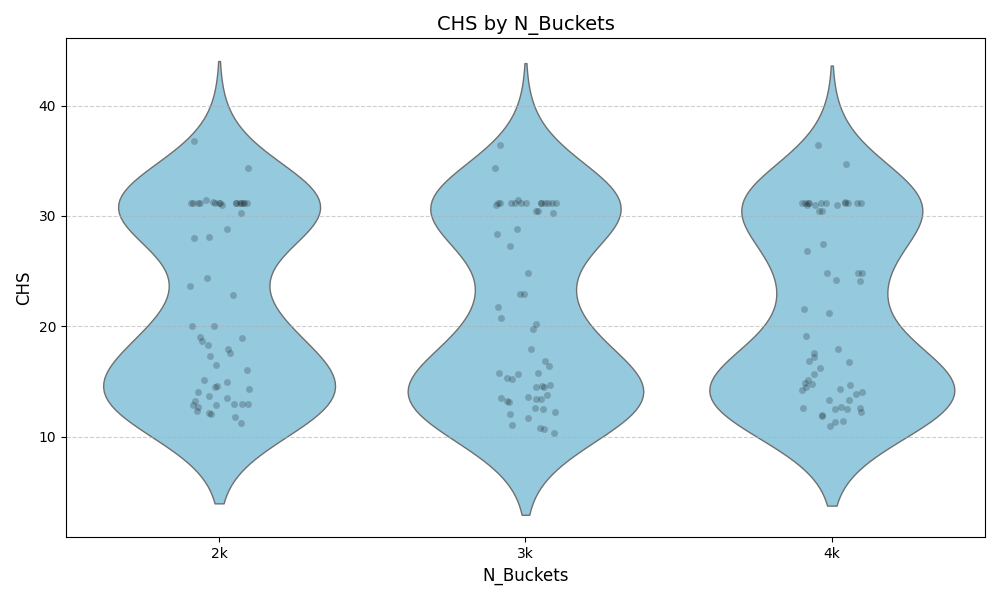
\includegraphics[width=0.3\textwidth]{figures/GlobalKMeans/hepatitis_violin_N_Buckets_vs_CHS.png} & 
        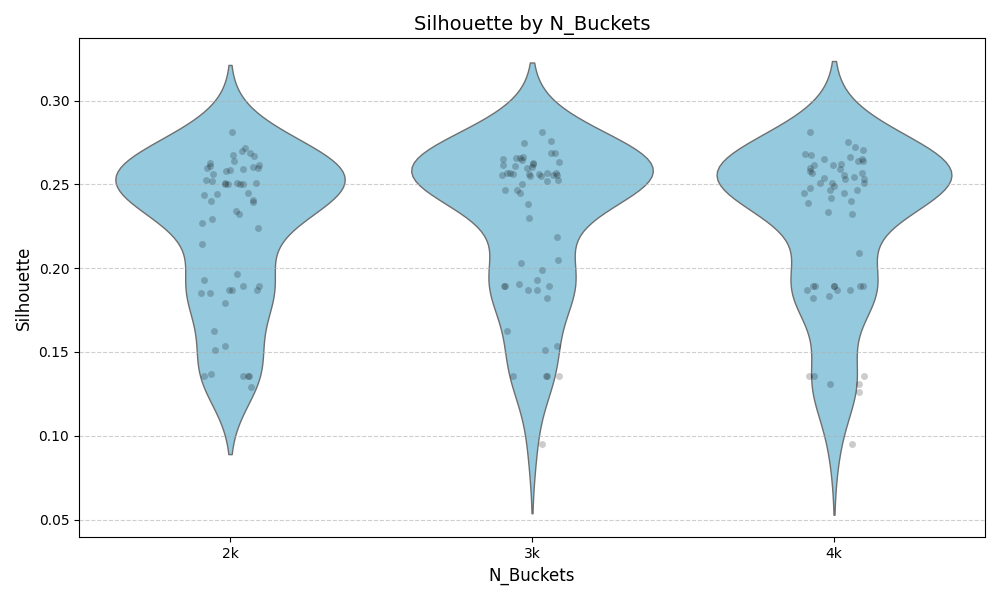
\includegraphics[width=0.3\textwidth]{figures/GlobalKMeans/mushroom_violin_N_Buckets_vs_Silhouette.png} & 
        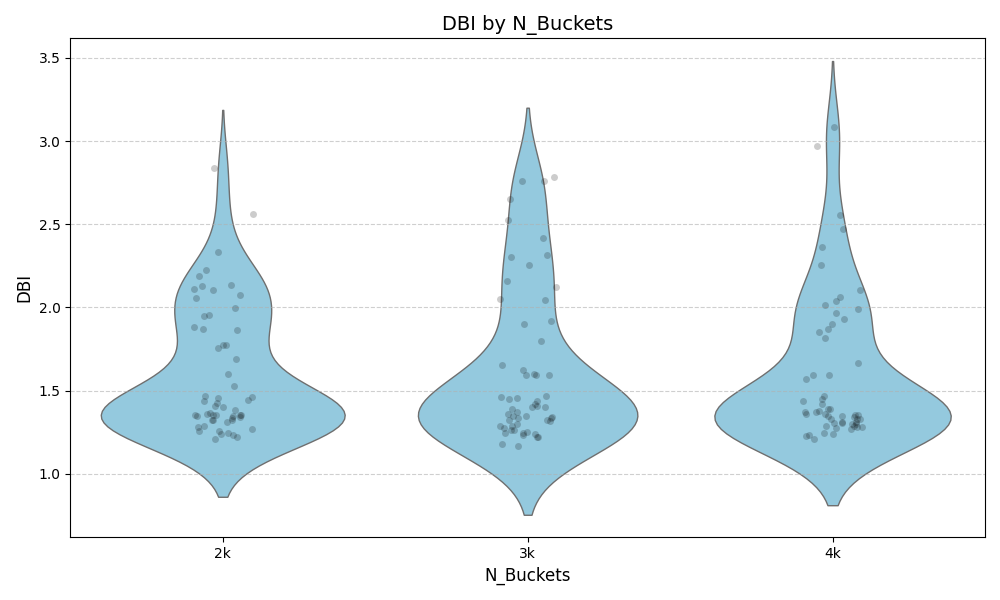
\includegraphics[width=0.3\textwidth]{figures/GlobalKMeans/penbased_violin_N_Buckets_vs_DBI.png} \\
    \end{tabular}
    \caption{Violin plots of the Global K-Means: Each row is a hyperparameter (k, distance metric, number of buckets), and each column is a dataset (Hepatitis, Mushroom, Pen-based)}
    \label{fig:globalkmeans:violin}
\end{figure}

\subsubsection{Best Runs}
As for the K-Means, we extracted for each of the datasets the run which achieved the best score for each of the metrics. A summary of them is displayed in Table \ref{tab:kmeans:best_runs}. For the sake of space efficiency, we shorten the names of the distance metrics to E (Euclidean), M (Manhattan) and C (Clark), and also we denote the number of buckets by N\_B.

\begin{table}[h!]
    \centering
    \begin{tabular}{|c|cccc|cccc|cccc|}
        \hline
                        & \multicolumn{4}{c|}{\textbf{Hepatitis}} & \multicolumn{4}{c|}{\textbf{Mushroom}} & \multicolumn{4}{c|}{\textbf{Pen-based}} \\ \hline
        \textbf{Metric} & \textbf{k} & \textbf{Dist.} & \textbf{N\_B} & \textbf{Value} 
                        & \textbf{k} & \textbf{Dist.} & \textbf{N\_B} & \textbf{Value}
                        & \textbf{k} & \textbf{Dist.} & \textbf{N\_B} & \textbf{Value} \\ \hline
        ARI            & 4          & C         & 2k      & 0.36
                       & 2          & C         & 2k        & 0.40
                       & 14          & E             & 4k       & 0.62 \\ \hline
        NMI            & 4          & C             & 2k        & 0.25
                       & 20          & M         & 3k       & 0.38 
                       & 20          & E         & 2k       & 0.73 \\ \hline
        DBI            & 20         & E         & 3k        & 1.27
                       & 2         & E             & 2k     & 1.20 
                       & 9         & E         & 3k     & 1.17 \\ \hline
        Silhouette     & 2          & M         & 2k        & 0.21
                       & 2          & E         & 2k        & 0.28
                       & 12          & E             & 3k       & 0.33 \\ \hline
        CHS            & 2          & E         & 2k        & 36.77
                       & 2          & E         & 2k        & 2996.24 
                       & 4          & E         & 4k        & 3357.99 \\ \hline
    \end{tabular}
    \caption{Metrics with corresponding values, and hyperparameters for three datasets.}
    \label{tab:kmeans:best_runs}
\end{table}

From these results, we can make some deductions as to which are the best hyperparameter configurations of the Global K-Means for the 3 datasets:
\begin{enumerate}
    \item \textbf{Hepatitis:} Once again, we observe a trend towards low values of k, although this time it is slightly more doubious, with two appearances of k=4. As for the distance metric, the results, as for the K-Means algorithm, are inconclusive. It is clear, however, that the Global K-Means thrives with a lower number of buckets in the Hepatitis dataset, with almost all top configurations having N\_B=2k.
    \item \textbf{Mushroom:} We can observe once again that k=2 is dominant, as for the K-Means. On the other hand, the Euclidean distance seems to be the most effective, though it is now unclear from these results which of the other two follows (although it was very clear with the violin plots, Figure \ref{fig:globalkmeans:violin}). As for the number of buckets, it again seems that a lower number of them (2k) tends to be the best option for Mushroom.
    \item \textbf{Pen-based:} It is again unclear which value of k could be the optimal for Pen-based, but the k's seem to be slightly higher this time compared to the results of the K-Means (between 9 and 14, probably). The Euclidean distance metric still remain as the obvious choice for this dataset.  The number of buckets this time seems to benefit from having greater values than for the other datasets, having a couple of 3k and 4k appearances in the best runs.
\end{enumerate}
When we compare the metric values achieved by these runs to the best performing runs of the K-Means, we observe that the differences are minimal, being the most consistent improvement in the DBI metric (although the improvement is still very slight). This, along with the fact that all of the observed trends regarding hyperparameters repeat for the 2 algorithms, leads us to believe that the Global K-Means does not represent a significant improvement over the standard K-Means in terms of clustering performance.

However, the Global K-Means does provide a consistency factor that the K-Means lacks. By having a deterministic approach to centroid initilization, the Global K-Means can guarantee to provide results equally good as the best of the K-Means without taking the risk of randomness. We have observed in our experiments that (with the 2 computational improvements proposed in \cite{Likas2003}) the 171 configurations of the Global K-Means that we ran for each dataset took significantly less amount of computation time than the 570 runs that we tested for the K-Means.

Thus, our conclusion regarding the Global K-Means is that its use should be recommended over the standard K-Means whenever possible, since it essentially eliminates the risk of randomness at no apparent cost.

\textit{Note:} Since the resulting configurations are mostly similar to those of the K-Means, we do not display again the resulting clusters. These would be equivalent to those visualized in Figure \ref{fig:kmeans:clusters}.
